\documentclass[]{book}
\usepackage{lmodern}
\usepackage{amssymb,amsmath}
\usepackage{ifxetex,ifluatex}
\usepackage{fixltx2e} % provides \textsubscript
\ifnum 0\ifxetex 1\fi\ifluatex 1\fi=0 % if pdftex
  \usepackage[T1]{fontenc}
  \usepackage[utf8]{inputenc}
\else % if luatex or xelatex
  \ifxetex
    \usepackage{mathspec}
  \else
    \usepackage{fontspec}
  \fi
  \defaultfontfeatures{Ligatures=TeX,Scale=MatchLowercase}
\fi
% use upquote if available, for straight quotes in verbatim environments
\IfFileExists{upquote.sty}{\usepackage{upquote}}{}
% use microtype if available
\IfFileExists{microtype.sty}{%
\usepackage{microtype}
\UseMicrotypeSet[protrusion]{basicmath} % disable protrusion for tt fonts
}{}
\usepackage[margin=1in]{geometry}
\usepackage{hyperref}
\hypersetup{unicode=true,
            pdftitle={Custom Angular Modules},
            pdfauthor={Matt Vaughn},
            pdfborder={0 0 0},
            breaklinks=true}
\urlstyle{same}  % don't use monospace font for urls
\usepackage{natbib}
\bibliographystyle{apalike}
\usepackage{color}
\usepackage{fancyvrb}
\newcommand{\VerbBar}{|}
\newcommand{\VERB}{\Verb[commandchars=\\\{\}]}
\DefineVerbatimEnvironment{Highlighting}{Verbatim}{commandchars=\\\{\}}
% Add ',fontsize=\small' for more characters per line
\usepackage{framed}
\definecolor{shadecolor}{RGB}{248,248,248}
\newenvironment{Shaded}{\begin{snugshade}}{\end{snugshade}}
\newcommand{\KeywordTok}[1]{\textcolor[rgb]{0.13,0.29,0.53}{\textbf{#1}}}
\newcommand{\DataTypeTok}[1]{\textcolor[rgb]{0.13,0.29,0.53}{#1}}
\newcommand{\DecValTok}[1]{\textcolor[rgb]{0.00,0.00,0.81}{#1}}
\newcommand{\BaseNTok}[1]{\textcolor[rgb]{0.00,0.00,0.81}{#1}}
\newcommand{\FloatTok}[1]{\textcolor[rgb]{0.00,0.00,0.81}{#1}}
\newcommand{\ConstantTok}[1]{\textcolor[rgb]{0.00,0.00,0.00}{#1}}
\newcommand{\CharTok}[1]{\textcolor[rgb]{0.31,0.60,0.02}{#1}}
\newcommand{\SpecialCharTok}[1]{\textcolor[rgb]{0.00,0.00,0.00}{#1}}
\newcommand{\StringTok}[1]{\textcolor[rgb]{0.31,0.60,0.02}{#1}}
\newcommand{\VerbatimStringTok}[1]{\textcolor[rgb]{0.31,0.60,0.02}{#1}}
\newcommand{\SpecialStringTok}[1]{\textcolor[rgb]{0.31,0.60,0.02}{#1}}
\newcommand{\ImportTok}[1]{#1}
\newcommand{\CommentTok}[1]{\textcolor[rgb]{0.56,0.35,0.01}{\textit{#1}}}
\newcommand{\DocumentationTok}[1]{\textcolor[rgb]{0.56,0.35,0.01}{\textbf{\textit{#1}}}}
\newcommand{\AnnotationTok}[1]{\textcolor[rgb]{0.56,0.35,0.01}{\textbf{\textit{#1}}}}
\newcommand{\CommentVarTok}[1]{\textcolor[rgb]{0.56,0.35,0.01}{\textbf{\textit{#1}}}}
\newcommand{\OtherTok}[1]{\textcolor[rgb]{0.56,0.35,0.01}{#1}}
\newcommand{\FunctionTok}[1]{\textcolor[rgb]{0.00,0.00,0.00}{#1}}
\newcommand{\VariableTok}[1]{\textcolor[rgb]{0.00,0.00,0.00}{#1}}
\newcommand{\ControlFlowTok}[1]{\textcolor[rgb]{0.13,0.29,0.53}{\textbf{#1}}}
\newcommand{\OperatorTok}[1]{\textcolor[rgb]{0.81,0.36,0.00}{\textbf{#1}}}
\newcommand{\BuiltInTok}[1]{#1}
\newcommand{\ExtensionTok}[1]{#1}
\newcommand{\PreprocessorTok}[1]{\textcolor[rgb]{0.56,0.35,0.01}{\textit{#1}}}
\newcommand{\AttributeTok}[1]{\textcolor[rgb]{0.77,0.63,0.00}{#1}}
\newcommand{\RegionMarkerTok}[1]{#1}
\newcommand{\InformationTok}[1]{\textcolor[rgb]{0.56,0.35,0.01}{\textbf{\textit{#1}}}}
\newcommand{\WarningTok}[1]{\textcolor[rgb]{0.56,0.35,0.01}{\textbf{\textit{#1}}}}
\newcommand{\AlertTok}[1]{\textcolor[rgb]{0.94,0.16,0.16}{#1}}
\newcommand{\ErrorTok}[1]{\textcolor[rgb]{0.64,0.00,0.00}{\textbf{#1}}}
\newcommand{\NormalTok}[1]{#1}
\usepackage{longtable,booktabs}
\usepackage{graphicx,grffile}
\makeatletter
\def\maxwidth{\ifdim\Gin@nat@width>\linewidth\linewidth\else\Gin@nat@width\fi}
\def\maxheight{\ifdim\Gin@nat@height>\textheight\textheight\else\Gin@nat@height\fi}
\makeatother
% Scale images if necessary, so that they will not overflow the page
% margins by default, and it is still possible to overwrite the defaults
% using explicit options in \includegraphics[width, height, ...]{}
\setkeys{Gin}{width=\maxwidth,height=\maxheight,keepaspectratio}
\IfFileExists{parskip.sty}{%
\usepackage{parskip}
}{% else
\setlength{\parindent}{0pt}
\setlength{\parskip}{6pt plus 2pt minus 1pt}
}
\setlength{\emergencystretch}{3em}  % prevent overfull lines
\providecommand{\tightlist}{%
  \setlength{\itemsep}{0pt}\setlength{\parskip}{0pt}}
\setcounter{secnumdepth}{5}
% Redefines (sub)paragraphs to behave more like sections
\ifx\paragraph\undefined\else
\let\oldparagraph\paragraph
\renewcommand{\paragraph}[1]{\oldparagraph{#1}\mbox{}}
\fi
\ifx\subparagraph\undefined\else
\let\oldsubparagraph\subparagraph
\renewcommand{\subparagraph}[1]{\oldsubparagraph{#1}\mbox{}}
\fi

%%% Use protect on footnotes to avoid problems with footnotes in titles
\let\rmarkdownfootnote\footnote%
\def\footnote{\protect\rmarkdownfootnote}

%%% Change title format to be more compact
\usepackage{titling}

% Create subtitle command for use in maketitle
\newcommand{\subtitle}[1]{
  \posttitle{
    \begin{center}\large#1\end{center}
    }
}

\setlength{\droptitle}{-2em}
  \title{Custom Angular Modules}
  \pretitle{\vspace{\droptitle}\centering\huge}
  \posttitle{\par}
  \author{Matt Vaughn}
  \preauthor{\centering\large\emph}
  \postauthor{\par}
  \predate{\centering\large\emph}
  \postdate{\par}
  \date{2017-10-30}

\usepackage{booktabs}
\usepackage{amsthm}
\makeatletter
\def\thm@space@setup{%
  \thm@preskip=8pt plus 2pt minus 4pt
  \thm@postskip=\thm@preskip
}
\makeatother

\usepackage{amsthm}
\newtheorem{theorem}{Theorem}[chapter]
\newtheorem{lemma}{Lemma}[chapter]
\theoremstyle{definition}
\newtheorem{definition}{Definition}[chapter]
\newtheorem{corollary}{Corollary}[chapter]
\newtheorem{proposition}{Proposition}[chapter]
\theoremstyle{definition}
\newtheorem{example}{Example}[chapter]
\theoremstyle{definition}
\newtheorem{exercise}{Exercise}[chapter]
\theoremstyle{remark}
\newtheorem*{remark}{Remark}
\newtheorem*{solution}{Solution}
\begin{document}
\maketitle

{
\setcounter{tocdepth}{1}
\tableofcontents
}
\chapter{Introduction}\label{intro}

\section{Welcome}\label{welcome}

Welcome to the \texttt{Custom\ Angular\ Modules} guide. This is not just
another book about Angular. However, this book is not about teaching you
the basics of Angular or using Typescript. There are many resources out
there that you can access. The purpose of this book is to provide you
with guidance on how to use Angular Modules the right way. You need to
know how to use this fundamental element of Angular effectively so that
you do not waste any time and resources by doing it the wrong way.
Rewriting and/or refactoring applications is an expensive process. Your
application or startup doesn't have to be another failure statistic -
the Angular framework provides you with the tools you need. Let's learn
how to use one of them to create a killer app.

\section{No Excuse to Not Build It Right the First
Time}\label{no-excuse-to-not-build-it-right-the-first-time}

You should be able to build the application right the first time so that
you can create amazing solutions for your current projects, but also for
your future projects. If you need to leverage and reuse code that you
have already developed wthout doing the dredded copy/paste, you need to
\emph{learn how to create custom Angular Modules the right way}. Thanks
for reading this guide. You will find complete and detailed instructions
on how to create custom modules.

Before we get started though, you need to know and understand how
Angular Modules can work for you to create amazing applications. The
solutions you develop need to be of the highest quality - your career
and reputation depends on it. I want you to be successful. Ask these
questions about your code:

\begin{itemize}
\tightlist
\item
  Are my components and services \emph{testable} using testing
  frameworks?
\item
  Are my components and services \emph{extensible} and allow me to add
  features easily.
\item
  Are my components and services \emph{maintainable} to allow developers
  to be efficient.
\item
  Are my components and services \emph{sharable} to allow for efficient
  code reuse.
\end{itemize}

Don't be too sad if you answered \texttt{no} to any of the questions
above. It is not entirely your fault. When new tools and frameworks are
released there is a lot of excitement. You get the typical
\texttt{Hello\ World} applications and tutorials from all of the rock
star coders out there. When we are trying to learn new things, we
gravitate towards these tutorials, ebooks, videos, and blogs. However,
not many individuals are providing guidance on how to architect
solutions that are:

\begin{itemize}
\tightlist
\item
  testable
\item
  extensible
\item
  maintainable
\item
  sharable
\end{itemize}

No worries, this guide will teach you a valuable and essential lesson -
how to create Angular Modules. Modules help us to keep things simple,
use single responsibility and seperation of concerns principles.

\section{What You Will Learn}\label{what-you-will-learn}

As mentioned previously, the focus of this book is to provide guidance
on understanding and using Angular Modules effectively. If you are new
to Angular and/or Typescript, please see the Resources chapter of this
book.

Whether your an experienced or new Angular developer, it should be your
goal to know:

\begin{itemize}
\tightlist
\item
  Why modules are important in your application architecture and design.
\item
  How to create custom modules that can be developed as their own
  Angular libraries.
\item
  How to use your custom modules in other Angular applications.
\item
  How to create different types of modules that take care of application
  concerns, like:

  \begin{itemize}
  \tightlist
  \item
    Core and shared elements of your application.
  \item
    UI and application components.
  \item
    Infrastructure services (i.e., Logging, Http, Security) and domain
    feature services that are specific to the solution.
  \end{itemize}
\end{itemize}

This guide will provide you with additional resources so that you are
successful in implementing your own modules. You will have links to
GitHub.com projects that contains source code and examples. In addition,
there will be a set of video courses that walk you through the basics
and the advanced topics of Angular modules.

\chapter{What's the Problem with My
Modules?}\label{whats-the-problem-with-my-modules}

If you are not sure, you may already have a problem.

Angular is built from the ground up with modularity in mind. When you
examine the structure of an Angular application, you see that it is a
composite of many modules. If it were a pyramid, you would have the
\texttt{app.module} as the tip and all of the required core modules,
modules you import from the framework, npm packages loading modules, and
perhaps your custom feature modules.

\begin{verbatim}
"Technology should enable, not disable, right?"
\end{verbatim}

The Angular team has given the developer community an awesome framework.
However, having a garage full of the best tools is of no use if you do
not know how to use them the right way.

\section{How do Angular Modules
work?}\label{how-do-angular-modules-work}

Angular applications really only need one module to be a functional
single page application. However, would you buy a house with only 4
walls - I guess it's kind of funtional, but not very useful. Different
rooms in a house provide the ability to organize and enable specialized
functionality for each room. The kitchen is very different from the
laundry room - and you would rather sleep in a bedroom instead of the
garage, right?

It is the same with Angular Modules, you can use them to organize your
code and provide specific features. Code modularity is very much in line
with the
\href{https://en.wikipedia.org/wiki/Single_responsibility_principle}{Singe
Responsibility Principle (SR)}. How many modules do you have in your
application?

The \href{https://angular.io/guide/ngmodule}{angular.io} site has more
details on what a \href{https://angular.io/api/core/NgModule}{module} is
and how they are used in a basic application. However, there doesn't
appear to be much guidance on how to implement modules or how to create
your own custom Angular modules. The purpose of the book is to provide
some guidance, not rules, on how to take advantage of Angular's
modularity. We will promote software development principles that make
sense and that also allow you to create solutions that are testable,
extensible, and very maintainable. The Angular team has given us a lot
of features - however, learning to use the most basic ones to their
capacity will serve us well.

\section{How Many Modules Do I Need?}\label{how-many-modules-do-i-need}

Now that we have some basic understanding on how modules work, you might
have some questions:

\begin{itemize}
\tightlist
\item
  Do I need more than one module?
\item
  Do I need to create and use custom modules?
\item
  What are the different types of modules that I should consider using?
\end{itemize}

\chapter{Why Create Angular Modules?}\label{why-create-angular-modules}

This section of the book will provide some reasons and motivation to use
Angular modules more fully. We've read or participated in developer
discussions about modularity and the benefits. Fundamentally, it is a
great concept. However, sometimes not so simple to implement in the real
world. It takes effort to understand and design applications. Modules
give you the mechanism to organize the \texttt{things} of your
application into containers. So that when combined or available from a
specified module container it makes sense. Modules also provide you with
some context of the feature set; in terms of how it is used and what it
does.

Modules are also very much in line with object-oriented programming
designs and patterns. These structures emphasize separating features of
a program, or features that can be distributed from distinct modules. A
module is a self-contained structure of related things. Modules also
help in the decomposition of applications into smaller pieces of
functionality
(\href{https://en.wikipedia.org/wiki/Separation_of_concerns}{SoC -
separation of concerns}).

\section{Modularity, Modularity, and
Modularity}\label{modularity-modularity-and-modularity}

The whole notion of modules is to create reusable items to improve
efficiency and minimize maintenance of source code. The base element of
an Angular application is a Module. Each Angular application contains an
app.module that is the entry point of the entire application.

Therefore, you are already familiar with using modules. Also, it is very
common to create additional modules in an Angular applications. However,
what if you want to create Angular modules that can be reused in more
than a single Angular application? Or, would you like to create custom
modules that can be published to NPM and shared with the world?

Think of modules as containers of related things. Even if you never
create a custom module that is distributable, you can still dramatically
improve the design of you existing Angular applications by creating
modules to encapsulate and organize specific feature sets. Angular
modules let you decide what items within the module are publicly
available. For example, if you create a module that contains an Angular
Service, it can act like an API that provides end-points to the
application to perform different actions. You get to use and implement
some nice architectural patterns that provide:

\begin{itemize}
\tightlist
\item
  A service facade pattern to provide end-points of functionality.
\item
  Abstract the implementation details to private members of the module.
\item
  Create a highly-testable service using specification tests.
\item
  Encapsulation of many items used to implement the feauture set.
\end{itemize}

\section{Reusable Angular Libraries}\label{reusable-angular-libraries}

You are already taking advantage of reusable Angular libraries in the
form of modules. The Angular team has encapsulated many of its feature
sets into distinct reusable libraries: modules. You simply reference and
import these modules into your application. The Angular team has created
the framework with infrastructure elements with amazing reusability -
the \texttt{@NgModule} mechanism. They use it internally to create many
of the usefule feature sets of Angular, such as:

\begin{Shaded}
\begin{Highlighting}[]
\ImportTok{import} \OperatorTok{\{}\NormalTok{ BrowserModule }\OperatorTok{\}} \ImportTok{from} \StringTok{'@angular/platform-browser'}\OperatorTok{;}
\ImportTok{import} \OperatorTok{\{}\NormalTok{ NgModule }\OperatorTok{\}} \ImportTok{from} \StringTok{'@angular/core'}\OperatorTok{;}
\ImportTok{import} \OperatorTok{\{}\NormalTok{ FormsModule }\OperatorTok{\}} \ImportTok{from} \StringTok{'@angular/forms'}\OperatorTok{;}
\ImportTok{import} \OperatorTok{\{}\NormalTok{ HttpModule }\OperatorTok{\}} \ImportTok{from} \StringTok{'@angular/http'}\OperatorTok{;}
\end{Highlighting}
\end{Shaded}

\section{Reuse Things Already
Developed}\label{reuse-things-already-developed}

You probably already have some candidates (Services, Components, etc.)
in mind that can be shared and reused in your applications.

\emph{Do not duplicate your code by copying to other places in your
applications. Bad things will find you eventually!}

Lt. Joe Kenda is a detective that had an amazing career in Colorado
Springs. He has solved literally hundreds of murder crimes. He is
pragmatic and he doesn't make mistakes. If Joe Kenda was a programmer,
he wouldn't cut and past code from another app.

\href{https://www.youtube.com/results?search_query=joe+kenda}{
\includegraphics{images/you-dont-get-a-do-over.jpg}}

For example, my team is now finishing up the second of two enterprise
Angular applications within 9 months. During the development of the
second application we noted that there were some things in the first
application that we wished we could use in the new application. And now
that we are finishing up the second application, there are even more
\texttt{elements} that we want to make reusable for future projects. The
best way to do this is to create reusable packages - custom Angular
modules.

Our current application takes advantage of using different kinds of
modules throughout the application. Now, we are going a step further by
creating modules that can be distributed and reused on more than a
single application. This is the next level of modularity. Do it now,
because you might not get the chance for a \texttt{do-over}!

\chapter{Scope of Solution}\label{scope-of-solution}

The scope or context of this information is creating custom modules that
contain reusable \texttt{elements} for Angular web applications. This
guide will demonstrate how to create a reusable module that contains
either services or components.

Just today our team designed a custom submit button that changes state
and shows a spinny icon while submitting to the back end of the
application. The problem with most buttons is when do you enable the
button to be submittable (when the form is valid, right?). And after you
have clicked the button, you want to restrict users from re-clicking the
Submit button.

Our new Submit button \texttt{component} can now be used by all forms in
different applications. But only, if we include it in our custom UI
module. Developing shared module packages allows you to create something
that can be used everywhere, but maintained in a single location. And
now, when you want to add more features to the component, add the
feature and bump the version number of the module. You now also have
backward compatibility for other applications using the older version.
Nice!

You will need to determine how you manage versions of the module if you
are not publishing to \url{https://www.npmjs.com/}. NPMjs already has
built-in version management for your NPM packages/modules.

\chapter{Tools}\label{tools}

The examples demonstrated will use
\href{https://code.visualstudio.com/download}{Visual Studio Code} and
other tools listed below to create the solution. Your development
environment should have the following installed and configured.

\begin{itemize}
\tightlist
\item
  node.js and npm

  \begin{itemize}
  \tightlist
  \item
    Download at: \url{https://nodejs.org/en/download/}
  \end{itemize}
\item
  Typescript

  \begin{itemize}
  \tightlist
  \item
    Install using npm: \texttt{npm\ install\ -g\ typescript}
  \end{itemize}
\end{itemize}

\section{Angular CLI}\label{angular-cli}

You are probably familiar with the Angular CLI tool - a command line
interface for Angular. More information at:
\url{https://cli.angular.io/}. It has many different features that allow
you to create new applications, build and service apps, testing,
linting, and formatting. You can also use to generate (or scaffold)
modules, services, components, classes, directives, interfaces and more.
You can get a lot of mileage out of tools like this.

\begin{Shaded}
\begin{Highlighting}[]
\NormalTok{npm install }\OperatorTok{-}\NormalTok{g @angular/cli}
\end{Highlighting}
\end{Shaded}

\chapter{Getting Started}\label{getting-started}

Use the following steps to create a new module project. The instructions
provide enough details for you to create a module of (2) different
types. The \protect\hyperlink{ui-modules}{Module Resources section} has
information on creating (2) different types of modules - each has a
different responsibility within the architecture of the application.

\begin{enumerate}
\def\labelenumi{\arabic{enumi}.}
\tightlist
\item
  \protect\hyperlink{ui-modules}{UI Modules}
\item
  \protect\hyperlink{service-modules}{Service Modules}
\end{enumerate}

\section{Angular Application Folders}\label{angular-application-folders}

Within Visual Studio Code, open the Powershell Terminal. Change to a
directory where you want to create the module project. Create a folder
for the project.

\begin{verbatim}
mkdir ng-common
\end{verbatim}

\begin{figure}
\centering
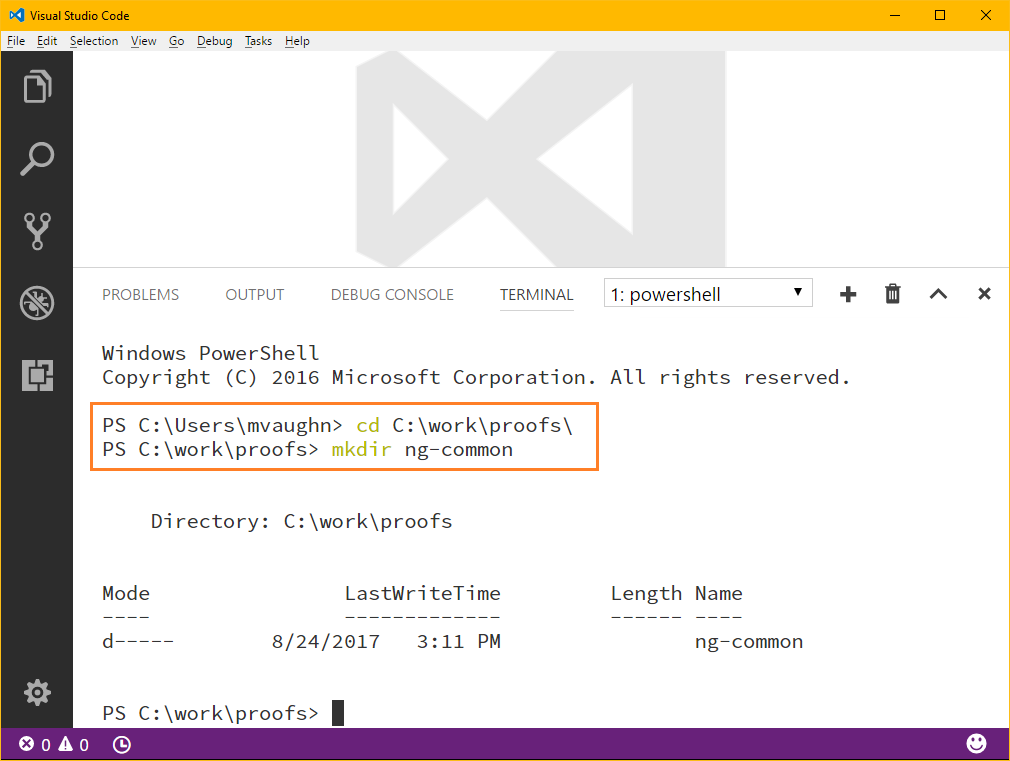
\includegraphics{images/create-module-folder.png}
\caption{}
\end{figure}

Now that we have a folder that will contain our module solution, open
the folder using the option from the File menu.

\begin{figure}
\centering
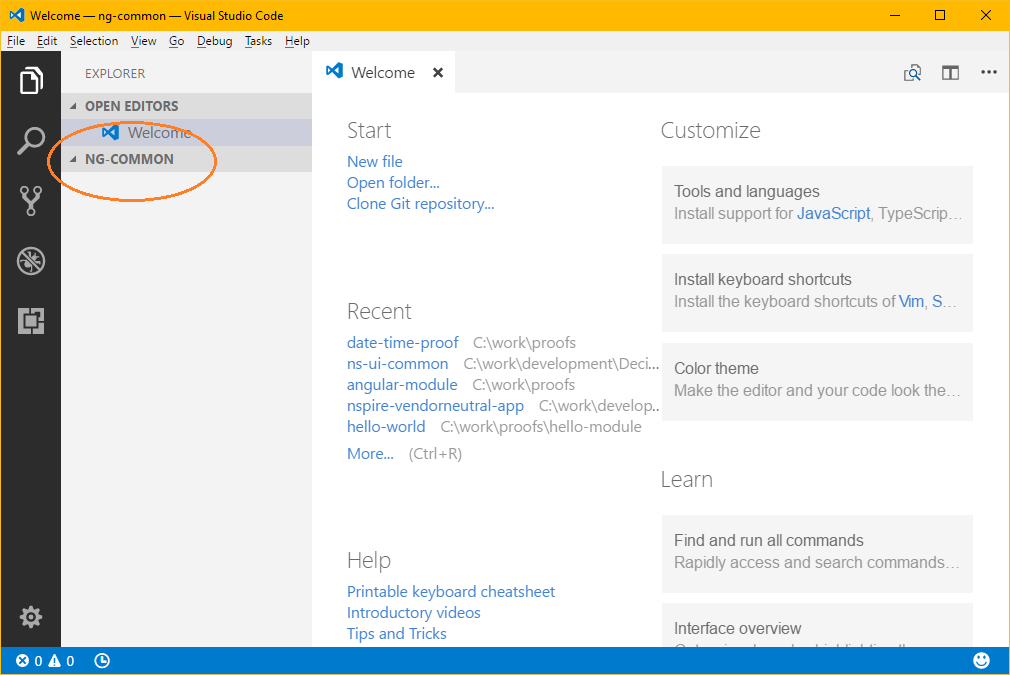
\includegraphics{images/open-module-folder.png}
\caption{}
\end{figure}

\subsection{Angular Folders}\label{angular-folders}

By convention, Angular web applications use a specific folder structure.
We also want to take advantage of the \texttt{angular-cli} tool to
generate code for our project. Therefore, we will create a
\texttt{src\textbackslash{}app} folder structure for the Angular members
of the project.

\section{Configuration Files}\label{configuration-files}

\subsection{index.ts}\label{index.ts}

This file is really the most important element of the solution. It will
allow you to publicly expose (can I say that in technical
documentation?) or allow clients to find the specified module of the
package - which is very important to Angular applications.

The only project member we need to expose is the module itself. The
\texttt{module} will actually define what elements of the module are
publicly visible - more on that later.

\begin{figure}
\centering
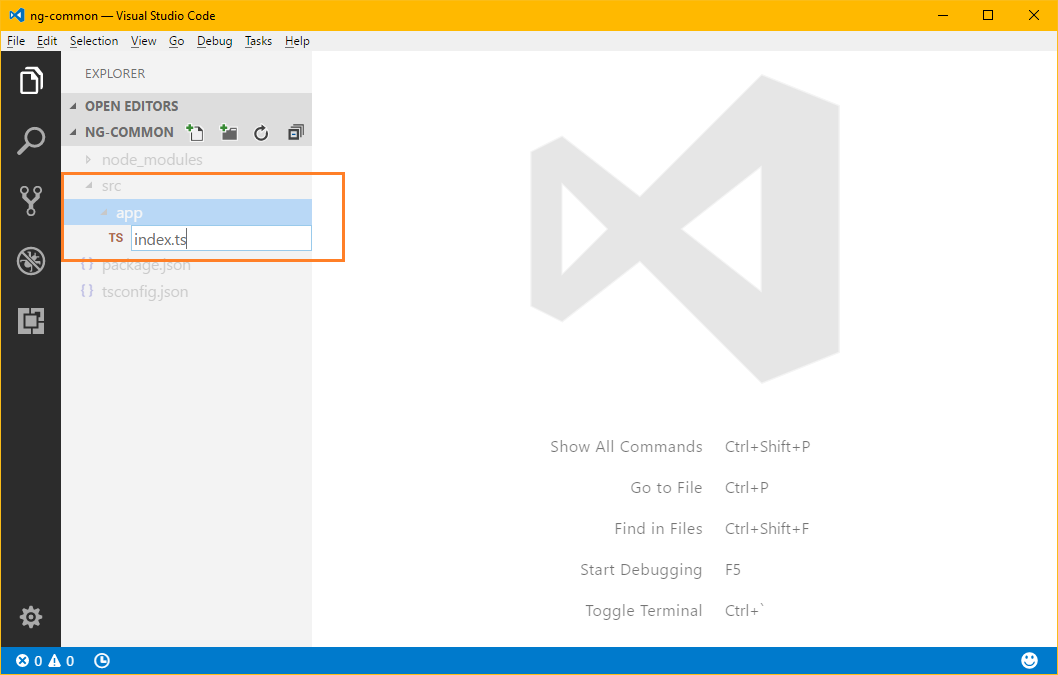
\includegraphics{images/create-index-file.png}
\caption{}
\end{figure}

\subsection{package.json}\label{package.json}

We will use a \texttt{package.json} file to set name, version, and also
to reference package dependencies required for the module.

Open the Powershell Terminal and run the following command. This will
create the \texttt{package.json} file.

\begin{verbatim}
npm init
\end{verbatim}

The \texttt{npm\ init} command creates a new \texttt{package.json} file
after guiding through a few prompts for information about the package.
This file is required when you want to use and or publish your package.

The complete/revised full version of the \texttt{package.json} file.

\begin{Shaded}
\begin{Highlighting}[]
\OperatorTok{\{}
  \StringTok{"name"}\OperatorTok{:} \StringTok{"StarterModule"}\OperatorTok{,}
  \StringTok{"version"}\OperatorTok{:} \StringTok{"2.1.1"}\OperatorTok{,}
  \StringTok{"description"}\OperatorTok{:} \StringTok{"asdf"}\OperatorTok{,}
  \StringTok{"main"}\OperatorTok{:} \StringTok{"index.js"}\OperatorTok{,}
  \StringTok{"scripts"}\OperatorTok{:} \OperatorTok{\{}
    \StringTok{"transpile"}\OperatorTok{:} \StringTok{"ngc"}\OperatorTok{,}
    \StringTok{"build"}\OperatorTok{:} \StringTok{"npm run transpile"}
  \OperatorTok{\},}
  \StringTok{"repository"}\OperatorTok{:} \OperatorTok{\{}
    \StringTok{"type"}\OperatorTok{:} \StringTok{"git"}\OperatorTok{,}
    \StringTok{"url"}\OperatorTok{:} \StringTok{"git+https://github.com/buildmotion/angular-module-starter.git"}
  \OperatorTok{\},}
  \StringTok{"author"}\OperatorTok{:} \StringTok{""}\OperatorTok{,}
  \StringTok{"license"}\OperatorTok{:} \StringTok{"MIT"}\OperatorTok{,}
  \StringTok{"bugs"}\OperatorTok{:} \OperatorTok{\{}
    \StringTok{"url"}\OperatorTok{:} \StringTok{"https://github.com/buildmotion/angular-module-starter/issues"}
  \OperatorTok{\},}
  \StringTok{"homepage"}\OperatorTok{:} \StringTok{"https://github.com/buildmotion/angular-module-starter#readme"}\OperatorTok{,}
  \StringTok{"devDependencies"}\OperatorTok{:} \OperatorTok{\{}
    \StringTok{"@angular/cli"}\OperatorTok{:} \StringTok{"^1.4.1"}\OperatorTok{,}
    \StringTok{"@angular/common"}\OperatorTok{:} \StringTok{"^4.4.0-RC.0"}\OperatorTok{,}
    \StringTok{"@angular/compiler"}\OperatorTok{:} \StringTok{"^4.4.0-RC.0"}\OperatorTok{,}
    \StringTok{"@angular/compiler-cli"}\OperatorTok{:} \StringTok{"^4.4.0-RC.0"}\OperatorTok{,}
    \StringTok{"@angular/core"}\OperatorTok{:} \StringTok{"^4.4.0-RC.0"}\OperatorTok{,}
    \StringTok{"rxjs"}\OperatorTok{:} \StringTok{"^5.0.1"}
  \OperatorTok{\}}
\OperatorTok{\}}
\end{Highlighting}
\end{Shaded}

\subsection{tsconfig.json}\label{tsconfig.json}

The next section is very important. Important. Typically, you would
compile a Typescript project using \texttt{tsc} - most of these
applications contain a \texttt{tsconfig.json} file that contains the
configuration for the build process. We are going to do much the same.
However, we are going to use the \texttt{ngc} - the ng compiler tool
with its own configuration. The \texttt{ngc} is located at:
\texttt{.\textbackslash{}node\_modules\textbackslash{}.bin\textbackslash{}ngc}.

Use the command below to create a new \texttt{tsconfig.json} file in the
root of the project. We will need to update the configuration using the
code snippet below.

\begin{Shaded}
\begin{Highlighting}[]
\NormalTok{tsc }\OperatorTok{--}\NormalTok{init}
\end{Highlighting}
\end{Shaded}

Open the \texttt{tsconfig.json} file and update the configuration using
the configuration in the snippet below.

\begin{Shaded}
\begin{Highlighting}[]
\OperatorTok{\{}
  \StringTok{"compilerOptions"}\OperatorTok{:} \OperatorTok{\{}
    \StringTok{"baseUrl"}\OperatorTok{:} \StringTok{"."}\OperatorTok{,}
    \StringTok{"declaration"}\OperatorTok{:} \KeywordTok{true}\OperatorTok{,}
    \StringTok{"experimentalDecorators"}\OperatorTok{:} \KeywordTok{true}\OperatorTok{,}
    \StringTok{"inlineSources"}\OperatorTok{:} \KeywordTok{true}\OperatorTok{,}
    \StringTok{"lib"}\OperatorTok{:}\NormalTok{ [}
      \StringTok{"es2015"}\OperatorTok{,}
      \StringTok{"dom"}
\NormalTok{    ]}\OperatorTok{,}
    \StringTok{"module"}\OperatorTok{:} \StringTok{"es2015"}\OperatorTok{,}
    \StringTok{"moduleResolution"}\OperatorTok{:} \StringTok{"node"}\OperatorTok{,}
    \StringTok{"noImplicitAny"}\OperatorTok{:} \KeywordTok{true}\OperatorTok{,}
    \StringTok{"outDir"}\OperatorTok{:} \StringTok{"dist"}\OperatorTok{,}
    \StringTok{"paths"}\OperatorTok{:} \OperatorTok{\{}
      \StringTok{"@angular/core"}\OperatorTok{:}\NormalTok{ [}
        \StringTok{"node_modules/@angular/core"}
\NormalTok{      ]}\OperatorTok{,}
      \StringTok{"rxjs/*"}\OperatorTok{:}\NormalTok{ [}
        \StringTok{"node_modules/rxjs/*"}
\NormalTok{      ]}
    \OperatorTok{\},}
    \StringTok{"rootDir"}\OperatorTok{:} \StringTok{"src/app"}\OperatorTok{,}
    \StringTok{"skipLibCheck"}\OperatorTok{:} \KeywordTok{true}\OperatorTok{,}
    \StringTok{"sourceMap"}\OperatorTok{:} \KeywordTok{true}\OperatorTok{,}
    \StringTok{"strictNullChecks"}\OperatorTok{:} \KeywordTok{true}\OperatorTok{,}
    \StringTok{"stripInternal"}\OperatorTok{:} \KeywordTok{true}\OperatorTok{,}
    \StringTok{"target"}\OperatorTok{:} \StringTok{"es5"}\OperatorTok{,}
  \OperatorTok{\},}
  \StringTok{"files"}\OperatorTok{:}\NormalTok{ [}
    \StringTok{"./src/app/index.ts"}
\NormalTok{  ]}\OperatorTok{,}
  \StringTok{"angularCompilerOptions"}\OperatorTok{:} \OperatorTok{\{}
    \StringTok{"strictMetadataEmit"}\OperatorTok{:} \KeywordTok{true}
  \OperatorTok{\}}
\OperatorTok{\}}
\end{Highlighting}
\end{Shaded}

For better build automation, you can update your \texttt{package.json}
file to include the code below. Notice that we are indicating that the
transpile should be performed by the \texttt{ngc} - the Angular compiler
tool. This tool is located at .

\begin{Shaded}
\begin{Highlighting}[]
\StringTok{"transpile"}\OperatorTok{:} \StringTok{"ngc"}\OperatorTok{,}
\StringTok{"build"}\OperatorTok{:} \StringTok{"npm run transpile"}
\end{Highlighting}
\end{Shaded}

Full sample of the \texttt{package.json} configuration.

\begin{Shaded}
\begin{Highlighting}[]
\OperatorTok{\{}
  \StringTok{"name"}\OperatorTok{:} \StringTok{"StarterModule"}\OperatorTok{,}
  \StringTok{"version"}\OperatorTok{:} \StringTok{"2.1.1"}\OperatorTok{,}
  \StringTok{"description"}\OperatorTok{:} \StringTok{""}\OperatorTok{,}
  \StringTok{"main"}\OperatorTok{:} \StringTok{"index.js"}\OperatorTok{,}
  \StringTok{"scripts"}\OperatorTok{:} \OperatorTok{\{}
    \StringTok{"transpile"}\OperatorTok{:} \StringTok{"ngc"}\OperatorTok{,}
    \StringTok{"build"}\OperatorTok{:} \StringTok{"npm run transpile"}
  \OperatorTok{\},}
  \StringTok{"repository"}\OperatorTok{:} \OperatorTok{\{}
    \StringTok{"type"}\OperatorTok{:} \StringTok{"git"}\OperatorTok{,}
    \StringTok{"url"}\OperatorTok{:} \StringTok{"git+https://github.com/buildmotion/angular-module-starter.git"}
  \OperatorTok{\},}
  \StringTok{"author"}\OperatorTok{:} \StringTok{""}\OperatorTok{,}
  \StringTok{"license"}\OperatorTok{:} \StringTok{"MIT"}\OperatorTok{,}
  \StringTok{"bugs"}\OperatorTok{:} \OperatorTok{\{}
    \StringTok{"url"}\OperatorTok{:} \StringTok{"https://github.com/buildmotion/angular-module-starter/issues"}
  \OperatorTok{\},}
  \StringTok{"homepage"}\OperatorTok{:} \StringTok{"https://github.com/buildmotion/angular-module-starter#readme"}\OperatorTok{,}
  \StringTok{"devDependencies"}\OperatorTok{:} \OperatorTok{\{}
    \StringTok{"@angular/cli"}\OperatorTok{:} \StringTok{"^1.4.1"}\OperatorTok{,}
    \StringTok{"@angular/common"}\OperatorTok{:} \StringTok{"^4.4.0-RC.0"}\OperatorTok{,}
    \StringTok{"@angular/compiler"}\OperatorTok{:} \StringTok{"^4.4.0-RC.0"}\OperatorTok{,}
    \StringTok{"@angular/compiler-cli"}\OperatorTok{:} \StringTok{"^4.4.0-RC.0"}\OperatorTok{,}
    \StringTok{"@angular/core"}\OperatorTok{:} \StringTok{"^4.4.0-RC.0"}\OperatorTok{,}
    \StringTok{"rxjs"}\OperatorTok{:} \StringTok{"^5.0.1"}
  \OperatorTok{\}}
\OperatorTok{\}}
\end{Highlighting}
\end{Shaded}

Use the Powershell terminal to build with the command below. This will
build and put the output files into the \texttt{dist} folder.

\begin{Shaded}
\begin{Highlighting}[]
\NormalTok{npm run build}
\end{Highlighting}
\end{Shaded}

\subsection{Compiler Options}\label{compiler-options}

There are quite a few compiler options available. Update the new
\texttt{tsconfig.json} file with the following configuration shown
below. Find more information about options here:
\href{https://www.typescriptlang.org/docs/handbook/compiler-options.html}{Typescript
Compiler Options}

\begin{itemize}
\tightlist
\item
  \textbf{declaration}: Generates corresponding .d.ts file.
\item
  \textbf{emitDecoratorMetadata}: Emit design-type metadata for
  decorated declarations in source.
\item
  \textbf{experimentalDecorators}: Enables experimental support for ES
  decorators.
\item
  \textbf{inlineSources}: Emit the source alongside the sourcemaps
  within a single file; requires --inlineSourceMap or --sourceMap to be
  set.
\item
  \textbf{mapRoot}: Specifies the location where debugger should locate
  map files instead of generated locations. Use this flag if the .map
  files will be located at run-time in a different location than the .js
  files. The location specified will be embedded in the sourceMap to
  direct the debugger where the map files will be located.
\item
  \textbf{module}: Specify module code generation.
\item
  \textbf{moduleResolution}: Determine how modules get resolved. Either
  ``Node'' for Node.js/io.js style resolution, or ``Classic''. See
  Module Resolution documentation for more details.
\item
  \textbf{noEmitOnError}: Do not emit outputs if any errors were
  reported.
\item
  \textbf{noImplicitAny}: Raise error on expressions and declarations
  with an implied any type.
\item
  \textbf{outDir}: Redirect output structure to the directory.
\item
  \textbf{rootDir}: Specifies the root directory of input files. Only
  use to control the output directory structure with --outDir.
\item
  \textbf{sourceMap}: Generates corresponding .map file.
\item
  \textbf{target}: Specify ECMAScript target version.
\end{itemize}

\section{angular-cli.json}\label{angular-cli.json}

Create/Add a new file called \texttt{angular-cli.json} in the root of
the project folder. Add the following contents.

You may need to update the \texttt{project.name} value to the name of
the current module project you are working on.

\begin{Shaded}
\begin{Highlighting}[]
\OperatorTok{\{}
    \StringTok{"project"}\OperatorTok{:} \OperatorTok{\{}
        \StringTok{"version"}\OperatorTok{:} \StringTok{"1.0.0"}\OperatorTok{,}
        \StringTok{"name"}\OperatorTok{:} \StringTok{"ng-common"}
    \OperatorTok{\},}
    \StringTok{"apps"}\OperatorTok{:}\NormalTok{ [}
        \OperatorTok{\{}
            \StringTok{"tsconfig"}\OperatorTok{:} \StringTok{"tsconfig.json"}\OperatorTok{,}
            \StringTok{"mobile"}\OperatorTok{:} \KeywordTok{false}\OperatorTok{,}
            \StringTok{"root"}\OperatorTok{:} \StringTok{"src"}\OperatorTok{,}
            \StringTok{"prefix"}\OperatorTok{:} \StringTok{"app"}
        \OperatorTok{\}}
\NormalTok{    ]}\OperatorTok{,}
    \StringTok{"defaults"}\OperatorTok{:} \OperatorTok{\{}
        \StringTok{"styleExt"}\OperatorTok{:} \StringTok{"css"}\OperatorTok{,}
        \StringTok{"prefixInterfaces"}\OperatorTok{:} \KeywordTok{false}\OperatorTok{,}
        \StringTok{"lazyRoutePrefix"}\OperatorTok{:} \StringTok{"+"}
    \OperatorTok{\}}
\OperatorTok{\}}
\end{Highlighting}
\end{Shaded}

\section{Install NPM Packages}\label{install-npm-packages}

Since our module is for sharing common Angular components, we will
install the following packages. Use the Powershell Terminal to run the
following commands.

\begin{verbatim}
npm install --save --save-dev rxjs@^5.0.1
npm install --save --save-dev @angular/cli@latest   
npm install --save --save-dev @angular/core 
npm install --save --save-dev @angular/common
npm install --save --save-dev @angular/compiler
npm install --save --save-dev @angular/compiler-cli
\end{verbatim}

Note, that the packages are only installed in the
\texttt{devDependencies} section of the \texttt{packages.json} file. We
only require the elements for development - we expect that the client
Angular application will have the required package references in the
\texttt{dependencies} of its packages.json file.

\begin{figure}
\centering
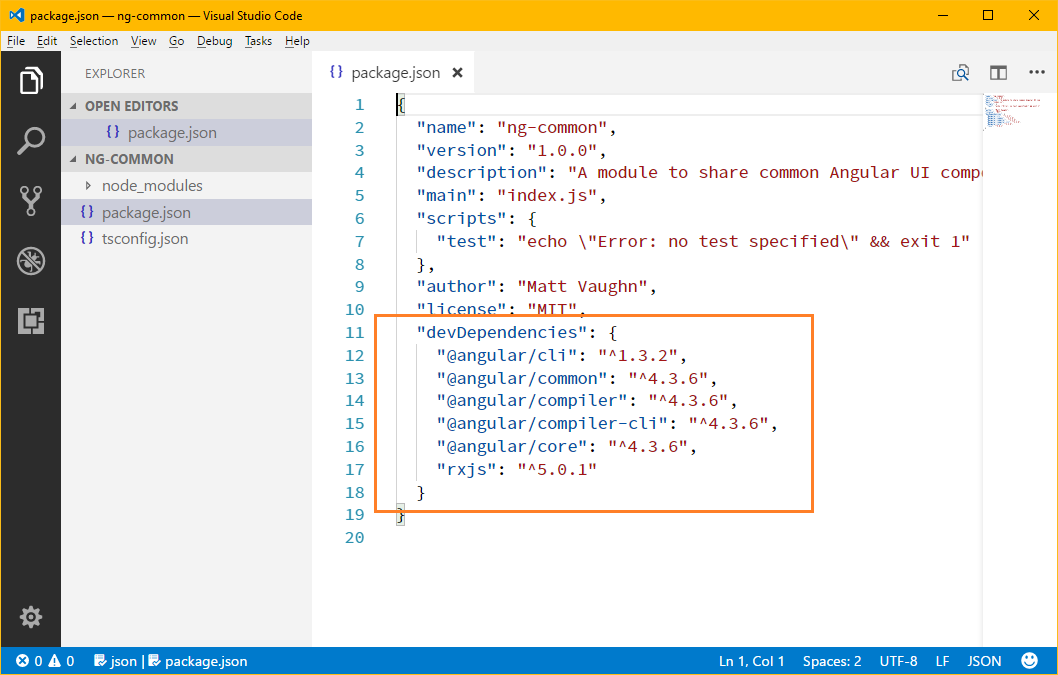
\includegraphics{images/ng-dev-dependencies.png}
\caption{}
\end{figure}

\chapter{Create a Module}\label{create-a-module}

Now, the moment that we have been waiting for. Create a module that will
provide access to all of the shared members (components, services, etc.)
we'll create later.

Run the following command to create a new module with the name
\texttt{ngCommonModule}. Note that you do not have to include the
\texttt{Module} suffix. The angular-cli tool will do that for you by
convention.

\begin{Shaded}
\begin{Highlighting}[]
\NormalTok{syntax}\OperatorTok{:}\NormalTok{ ng generate module }\OperatorTok{<}\NormalTok{NAME}\OperatorTok{-}\NormalTok{OF}\OperatorTok{-}\NormalTok{YOUR}\OperatorTok{-}\NormalTok{MODULE}\OperatorTok{>}
\NormalTok{example}\OperatorTok{:}\NormalTok{ ng generate module ngCommon}
\end{Highlighting}
\end{Shaded}

\begin{figure}
\centering
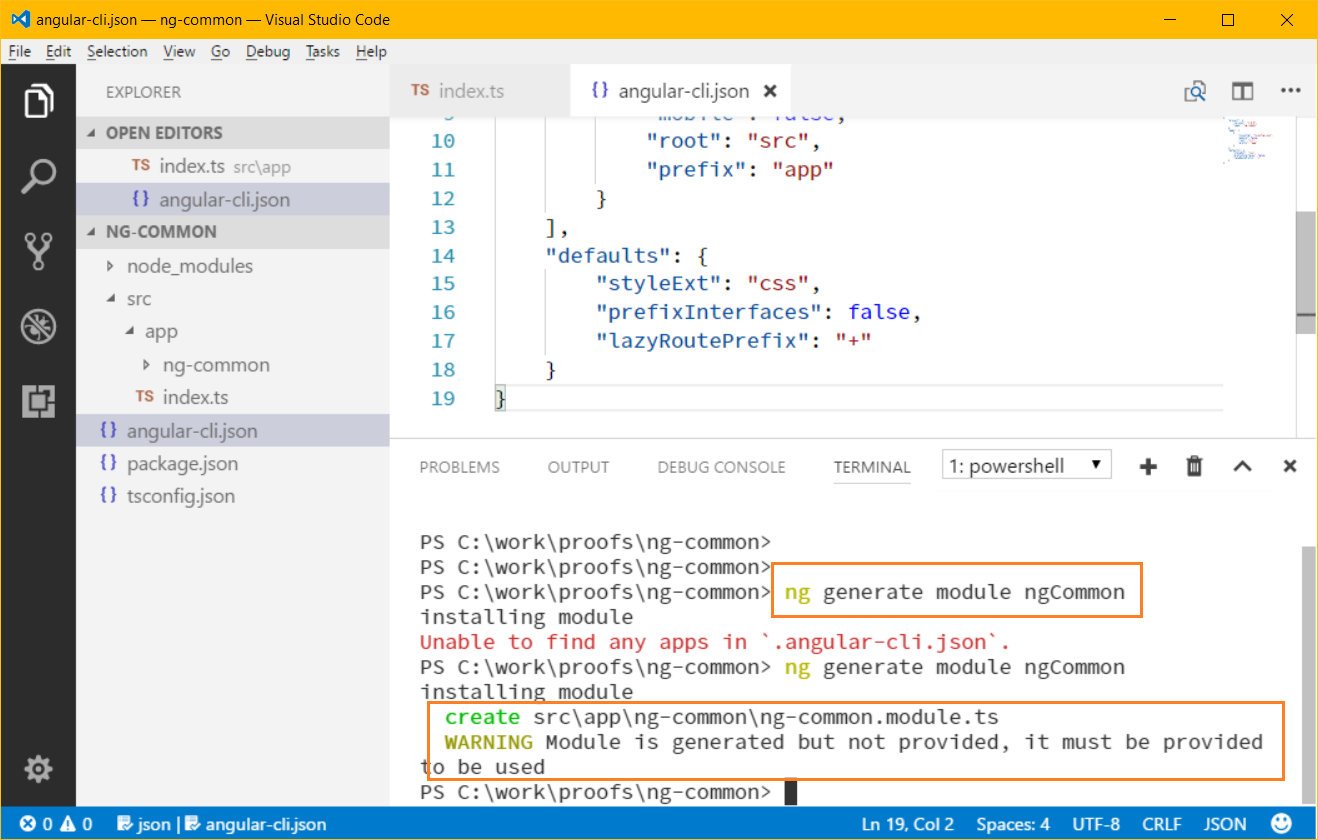
\includegraphics{images/ng-generate-module.png}
\caption{}
\end{figure}

\section{Module Configuration}\label{module-configuration}

We will use the \texttt{@NgModule} declaration to add imported items to
the \texttt{imports}, \texttt{declarations}, and \texttt{exports}

\begin{Shaded}
\begin{Highlighting}[]
\ImportTok{import} \OperatorTok{\{}\NormalTok{ NgModule }\OperatorTok{\}} \ImportTok{from} \StringTok{'@angular/core'}\OperatorTok{;}
\ImportTok{import} \OperatorTok{\{}\NormalTok{ CommonModule }\OperatorTok{\}} \ImportTok{from} \StringTok{'@angular/common'}\OperatorTok{;}

\NormalTok{\textbackslash{}@}\AttributeTok{NgModule}\NormalTok{(}\OperatorTok{\{}
  \DataTypeTok{imports}\OperatorTok{:}\NormalTok{ [}
\NormalTok{    CommonModule}
\NormalTok{  ]}\OperatorTok{,}
  \DataTypeTok{declarations}\OperatorTok{:}\NormalTok{ []}
\OperatorTok{\}}\NormalTok{)}
\ImportTok{export} \KeywordTok{class}\NormalTok{ NgCommonModule }\OperatorTok{\{} \OperatorTok{\}}
\end{Highlighting}
\end{Shaded}

\subsection{Module Name}\label{module-name}

The default name of the module is created when the \texttt{package.json}
file is created. Now that we have a module and the client applications
will reference the module by name, you will need to update the
\texttt{name} setting in the \texttt{package.json} file before
publishing the module.

\begin{verbatim}
old: ng-common
new: NgCommonModule
\end{verbatim}

\emph{Note: Later we will copy the \texttt{package.json} file to the
output directory before publishing the module. The names should match in
both files. }

\begin{Shaded}
\begin{Highlighting}[]
\OperatorTok{\{}
  \StringTok{"name"}\OperatorTok{:} \StringTok{"NgCommonModule"}\OperatorTok{,}
  \StringTok{"version"}\OperatorTok{:} \StringTok{"1.1.1"}\OperatorTok{,}
  \StringTok{"description"}\OperatorTok{:} \StringTok{"A module to share common Angular UI components."}\OperatorTok{,}
  \StringTok{"main"}\OperatorTok{:} \StringTok{"index.js"}\OperatorTok{,}
  \StringTok{"scripts"}\OperatorTok{:} \OperatorTok{\{}
    \StringTok{"test"}\OperatorTok{:} \StringTok{"echo }\SpecialCharTok{\textbackslash{}"}\StringTok{Error: no test specified}\SpecialCharTok{\textbackslash{}"}\StringTok{ && exit 1"}
  \OperatorTok{\},}
  \StringTok{"author"}\OperatorTok{:} \StringTok{"Matt Vaughn"}\OperatorTok{,}
  \StringTok{"license"}\OperatorTok{:} \StringTok{"MIT"}\OperatorTok{,}
  \StringTok{"devDependencies"}\OperatorTok{:} \OperatorTok{\{}
    \StringTok{"@angular/cli"}\OperatorTok{:} \StringTok{"^1.3.2"}\OperatorTok{,}
    \StringTok{"@angular/common"}\OperatorTok{:} \StringTok{"^4.3.6"}\OperatorTok{,}
    \StringTok{"@angular/compiler"}\OperatorTok{:} \StringTok{"^4.3.6"}\OperatorTok{,}
    \StringTok{"@angular/compiler-cli"}\OperatorTok{:} \StringTok{"^4.3.6"}\OperatorTok{,}
    \StringTok{"@angular/core"}\OperatorTok{:} \StringTok{"^4.3.6"}\OperatorTok{,}
    \StringTok{"rxjs"}\OperatorTok{:} \StringTok{"^5.0.1"}
  \OperatorTok{\}}
\OperatorTok{\}}
\end{Highlighting}
\end{Shaded}

\subsection{Export the Module}\label{export-the-module}

Add an \texttt{export} for the module in the \texttt{index.ts} file.
When the module project is compiled, this will create an
\texttt{index.js} file that is referenced as the \texttt{main} value in
the package.json file.

\begin{Shaded}
\begin{Highlighting}[]
\ImportTok{export} \OperatorTok{*} \ImportTok{from} \StringTok{'./ng-common/ng-common.module'}\OperatorTok{;}
\end{Highlighting}
\end{Shaded}

\emph{\textbf{NOTE}: Adding the \texttt{export} item for the module is
required. Otherwise, the Angular client application will throw an
exception stating that the ngCommonModule is not an @ngModule -
basically, it cannot find it due to not being exported and referenced in
the \texttt{index.js}.}

\section{Module Resources}\label{module-resources}

Now that we have a structure and process to create a module we are in a
better place. Now you need to start thinking about the contents of the
module.

\emph{Principle: A module should only contain related and like items
that as a composite make up the module contents. A module should not be
a }\textbf{``junk drawer''}\_ that contains non-related items. \_

For example, in our current Angular applications we have service and ui
modules. The \emph{UI modules} contain components, routes, pipes,
directives, and things related to the UI or display of content. We also
have \emph{service modules} that contain Angular services, business
logic code, HTTP services, rules and business actions. These services
basically contain the \emph{business logic} of the application to enable
a clear separation of concerns between the UI/UX and the business end of
the application.

My hope is that we can abstract the \emph{service modules} into separate
and reusable modules. One scenario is that the service modules have the
potential for reuse in other web and hybrid mobile applications. Another
benefit, is that the unit and/or specification testing of service
modules is simplified and targets/context of this type of testing is
much different that UI testing.

The next two sections talk about \emph{ui modules} and \emph{service
modules}. My opinion is that modules of these types should not be
combined into a single module

\hypertarget{ui-modules}{\subsection{\texorpdfstring{UI Modules:
Components and Angular
``Things''}{UI Modules: Components and Angular Things}}\label{ui-modules}}

Use the \texttt{angular-cli} to create a component. Note that we are
using the path \texttt{ng-common\textbackslash{}helloWorld} - this
allows the CLI to find and update the \texttt{ngCommonModule} with the
component configuration (Why write code when you don't have to?):

\begin{enumerate}
\def\labelenumi{\arabic{enumi}.}
\tightlist
\item
  import
\item
  declaration
\item
  export
\end{enumerate}

\begin{verbatim}
ng generate component ng-common\helloWorld
\end{verbatim}

\begin{figure}
\centering
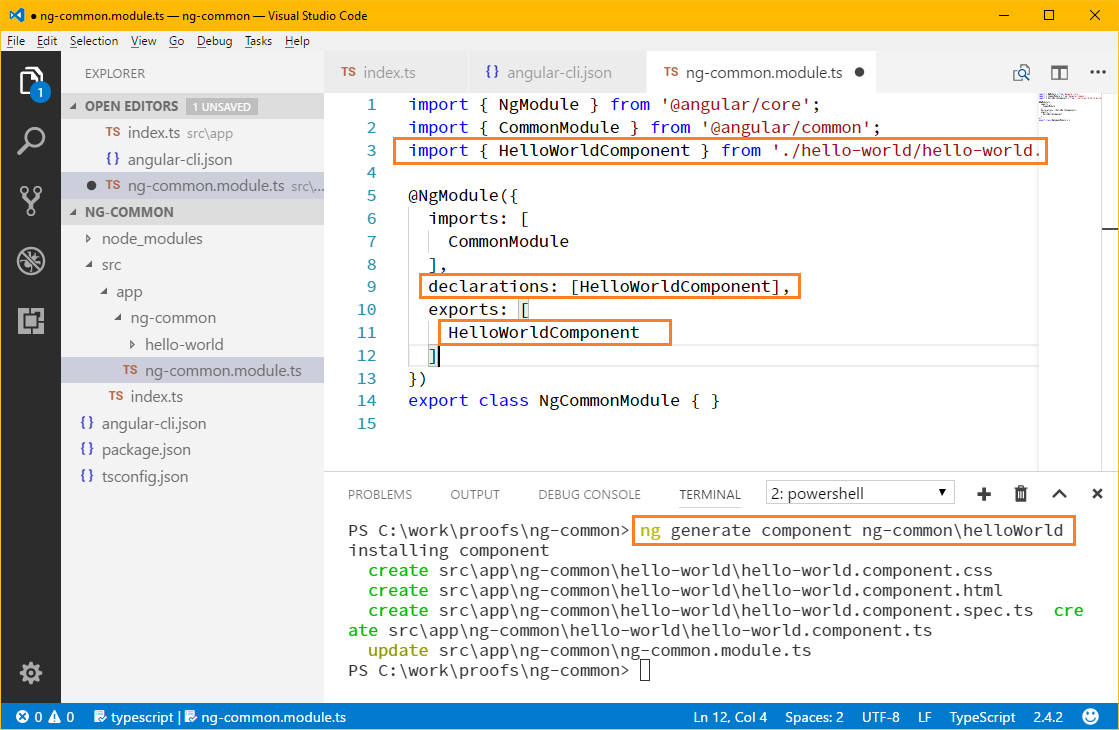
\includegraphics{images/ng-generate-component.png}
\caption{}
\end{figure}

\subsubsection{Declare and Export
Components}\label{declare-and-export-components}

If you want your components to be publicly exposed, or I should say
available (sounds better), you will need to add the component to the
\texttt{exports} array of the @ngModule.

Exporting, allows the component to be publicly available to applications
that import/use this module.

\begin{Shaded}
\begin{Highlighting}[]
\NormalTok{\textbackslash{}@}\AttributeTok{NgModule}\NormalTok{(}\OperatorTok{\{}
  \DataTypeTok{imports}\OperatorTok{:}\NormalTok{ [}
\NormalTok{    CommonModule}
\NormalTok{  ]}\OperatorTok{,}
  \DataTypeTok{declarations}\OperatorTok{:}\NormalTok{ [HelloWorldComponent]}\OperatorTok{,}
  \DataTypeTok{exports}\OperatorTok{:}\NormalTok{ [}
\NormalTok{    HelloWorldComponent}
\NormalTok{  ]}
\OperatorTok{\}}\NormalTok{)}
\end{Highlighting}
\end{Shaded}

\subsubsection{HelloWorldComponent}\label{helloworldcomponent}

The \texttt{HelloWorldComponent} is created in its own folder using the
same conventions we are used to when working with an Angular
application. We have:

\begin{itemize}
\tightlist
\item
  a \texttt{component} class with an \texttt{@Component} decorator.
\item
  an HTML file that will render when the \texttt{selector} is used.
\item
  a CSS file for styling the HTML.
\item
  a \texttt{specification\ test} file to write specification tests.
\end{itemize}

\begin{Shaded}
\begin{Highlighting}[]
\ImportTok{import} \OperatorTok{\{}\NormalTok{ Component}\OperatorTok{,}\NormalTok{ OnInit }\OperatorTok{\}} \ImportTok{from} \StringTok{'@angular/core'}\OperatorTok{;}

\NormalTok{@}\AttributeTok{Component}\NormalTok{(}\OperatorTok{\{}
  \DataTypeTok{selector}\OperatorTok{:} \StringTok{'app-hello-world'}\OperatorTok{,}
  \DataTypeTok{templateUrl}\OperatorTok{:} \StringTok{'./hello-world.component.html'}\OperatorTok{,}
  \DataTypeTok{styleUrls}\OperatorTok{:}\NormalTok{ [}\StringTok{'./hello-world.component.css'}\NormalTok{]}
\OperatorTok{\}}\NormalTok{)}
\ImportTok{export} \KeywordTok{class}\NormalTok{ HelloWorldComponent }\KeywordTok{implements}\NormalTok{ OnInit }\OperatorTok{\{}

  \AttributeTok{constructor}\NormalTok{() }\OperatorTok{\{} \OperatorTok{\}}

  \AttributeTok{ngOnInit}\NormalTok{() }\OperatorTok{\{}
  \OperatorTok{\}}

\OperatorTok{\}}
\end{Highlighting}
\end{Shaded}

\subsubsection{What to do about HTML and CSS
files?}\label{what-to-do-about-html-and-css-files}

In a typical Angular application, a component references the HTML and
CSS files in the \texttt{@Component} decorator. For shared module
packages (which are not Angular applications) it is best to include the
HTML and CSS as inline text in the \citet{Component} decorator.
Otherwise, you will need to implement a more elaborate build scheme that
will bundle and/or inline the file contents for you.

My opinion is that the Angular CLI should have the ability and feature
to create a stand alone module without requiring the context of being
within an Angular application. There are requests for this feature -
however, not much activity from the team managing the Angular CLI tool.
It is nice that we \emph{\textbf{CAN}} use the CLI to create feature and
service modules in existing Angular applications. But the point of even
having the concept of modules is that they can be reused and shared. If
they are stuck in the muck of a single application you have the
temptation of copying the folders/files into a new project. And if you
do that (I'm guilty of this from time to time), beware trouble is
lurking and it will find you!

\hypertarget{service-modules}{\subsection{Service Modules: Services,
Business Providers, Actions, and Rules\ldots{}}\label{service-modules}}

Use the information in this section if you building a \emph{service
module} - a module that is basically an entry point into your business
logic with a service API-like abstraction. The service APIs provide a
facade pattern implementation that delegate the real concrete business
logic in other classes below the service.

Each consumer of the service (most likely an Angular Component) will
only have direct access to the service of the module. Access to things
internal should not be allowed. For example, you do not want the
components to directly interact with or have access to:

\begin{itemize}
\tightlist
\item
  Business Providers
\item
  Business Actions*
\item
  Business Rules
\item
  Http Providers/Services that interact with the web services or Web
  APIs
\end{itemize}

Our web team has current standards, patterns, and practices for
implementing business logic in our Angular applications - we take
advantage of the
\href{https://www.npmjs.com/package/angular-actions}{angular-actions npm
package} along with the
\href{https://www.npmjs.com/package/angular-rules-engine}{angular-rules-engine}.
These packages elevate your business lgoic to the next level with a
robust processing framwork for business logic, authorization, business
rule process, data validation, and interaction with other services like
Angular HTTP.

\chapter{Compiling and Publishing the
Module}\label{compiling-and-publishing-the-module}

We now have a module with something that can be reused - everyone wants
the awesome \texttt{HelloWorldComponent}, right? You get the point - you
can now create as many reusable components as you want.

Let's compile something so we can use the module. Typically within
Visual Studio Code you can use the command below to run the build task.

\begin{Shaded}
\begin{Highlighting}[]
\NormalTok{SHIFT}\OperatorTok{+}\NormalTok{CTRL B}
\end{Highlighting}
\end{Shaded}

However, when we use this command, the tool asks you to select the
specified build task. Usually, the
\texttt{tsc:\ build\ -\ tsconfig.json} option from your
\texttt{tsconfig.json} file. This will work every time.

\begin{figure}
\centering
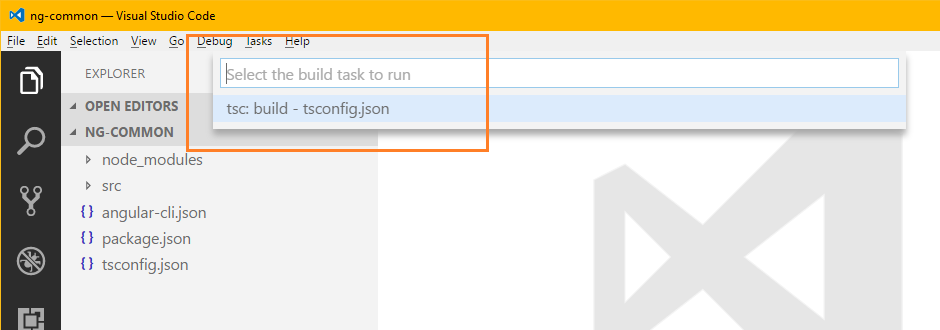
\includegraphics{images/select-build-task.png}
\caption{}
\end{figure}

\section{Alternate: Configure a Default Build
Task}\label{alternate-configure-a-default-build-task}

Use the \texttt{CTRL\ +\ P} command to show the command pallete. Enter
\texttt{task} to display the \texttt{Tasks} options. Select the
\texttt{Tasks:\ Configure\ Default\ Build\ Task}.

\begin{figure}
\centering
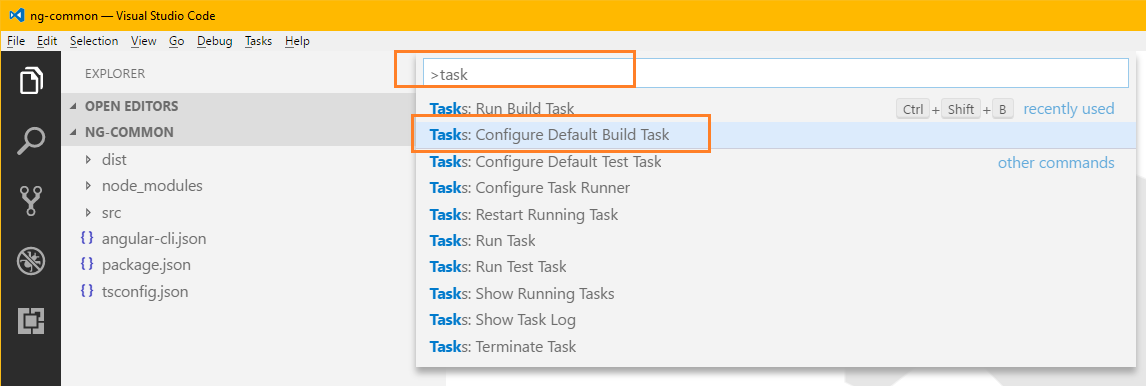
\includegraphics{images/configure-default-build-task.png}
\caption{}
\end{figure}

Select the option \texttt{tsc:\ build\ -tsconfig.json} as your option.
This will configure the task to use the \texttt{tsconfig.json} when
building the code with the \texttt{tsc} Typescript compiler.

\begin{figure}
\centering
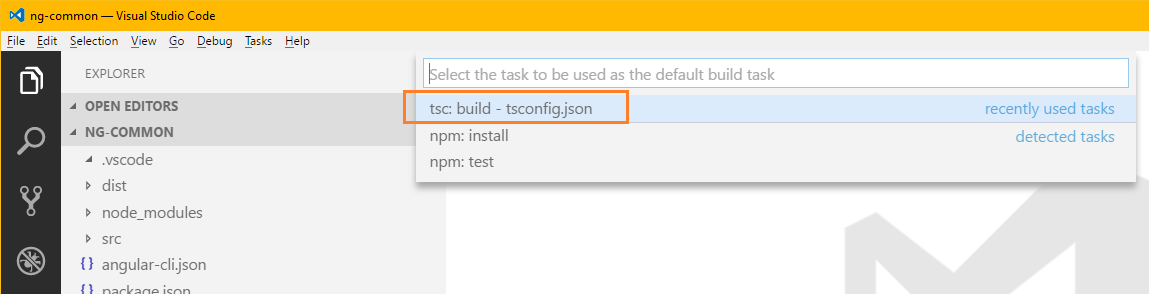
\includegraphics{images/select-default-task.png}
\caption{}
\end{figure}

This will create a \texttt{tasks.json} file in the .vscode folder of
your project.

\begin{Shaded}
\begin{Highlighting}[]
\OperatorTok{\{}
    \CommentTok{// See https://go.microsoft.com/fwlink/?LinkId=733558}
    \CommentTok{// for the documentation about the tasks.json format}
    \StringTok{"version"}\OperatorTok{:} \StringTok{"2.0.0"}\OperatorTok{,}
    \StringTok{"tasks"}\OperatorTok{:}\NormalTok{ [}
        \OperatorTok{\{}
            \StringTok{"type"}\OperatorTok{:} \StringTok{"typescript"}\OperatorTok{,}
            \StringTok{"tsconfig"}\OperatorTok{:} \StringTok{"tsconfig.json"}\OperatorTok{,}
            \StringTok{"problemMatcher"}\OperatorTok{:}\NormalTok{ [}
                \StringTok{"$tsc"}
\NormalTok{            ]}\OperatorTok{,}
            \StringTok{"group"}\OperatorTok{:} \OperatorTok{\{}
                \StringTok{"kind"}\OperatorTok{:} \StringTok{"build"}\OperatorTok{,}
                \StringTok{"isDefault"}\OperatorTok{:} \KeywordTok{true}
            \OperatorTok{\}}
        \OperatorTok{\}}
\NormalTok{    ]}
\OperatorTok{\}}
\end{Highlighting}
\end{Shaded}

\section{Compiled Output}\label{compiled-output}

The compiled output of the build is in the \texttt{dist} folder of the
project. The output directory is configured in the
\texttt{tsconfig.json}.\texttt{outDir} setting.

\section{Distribution package.json
Configuration}\label{distribution-package.json-configuration}

In order for other applications to use the module package, the module
must contain a \texttt{package.json} file. You can copy the
\texttt{package.json} file from the root of the project to the
\texttt{dist} folder.

The initial file should have a version of \texttt{1.0.0}. You may want
to modify the version of the module package when new features,
components, or bug fixes occur. You can use the \texttt{npm} command to
update the version:

\begin{Shaded}
\begin{Highlighting}[]
\NormalTok{Syntax}\OperatorTok{:}\NormalTok{ npm version [patch}\OperatorTok{|}\NormalTok{minor}\OperatorTok{|}\NormalTok{major]}
\NormalTok{npm version patch}
\NormalTok{npm version minor}
\NormalTok{npm version major}
\end{Highlighting}
\end{Shaded}

The following shows the usage of the npm command and the changes in the
version of the module package. How you use versioning is up to you
and/or your team. Please remember, that the version and how your package
is referenced by clients will have an impact on the applications that
will use your module.

Make sure that you are running the \texttt{npm\ version} command from
the \texttt{dist} folder so that the correct \texttt{package.json} file
is updated. Or, you may want to update the source file and have an XCOPY
process that copies the file to the \texttt{dist} folder during builds -
they should probably be kept in sync.

\begin{verbatim}
PS C:\work\proofs\ng-common>
PS C:\work\proofs\ng-common>
PS C:\work\proofs\ng-common> cd .\dist\
PS C:\work\proofs\ng-common\dist> npm version patch
v1.0.1
PS C:\work\proofs\ng-common\dist> npm version minor
v1.1.0
PS C:\work\proofs\ng-common\dist> npm version major
v2.0.0
\end{verbatim}

\chapter{Using the Module}\label{using-the-module}

In order to use the module, you will need to create or configure an
existing Angular web application. The most common way to use a package
module is to install it using
\texttt{npm\ install\ \textless{}myModuleName\textgreater{}}.

\begin{verbatim}
npm install angular-rules-engine@0.0.27 --save --save-dev
\end{verbatim}

This will work if you publish the package to an npm repository like
\url{https://www.npmjs.com/}. For modules that you want to share with
the world - this is a great way to do it.

For example, our team uses the
\href{https://www.npmjs.com/package/angular-rules-engine}{angular-rules-engine}
npm package developed and maintained by one of team members (me).

If you do not need to or do not want to make your module publicly
available, you can publish the contents of the \texttt{dist} folder from
the module project to a location accessible via file path/network share
to the Angular application under consideration.

For example, our team will publish modules to an \texttt{ng-resources}
folder. This folder can be version controlled and updated when and if
newer versions are made available. You can also create folders that have
\texttt{version} information so that you can maintain and use more than
one version of the module.

\section{Update package.json with Reference to
Module}\label{update-package.json-with-reference-to-module}

You can add a reference to the \texttt{devDependecies} and/or the
\texttt{dependencies} settings in the applications \texttt{package.json}
file.

\begin{verbatim}
"NgCommonModule": "../ng-resources/ng-common"
\end{verbatim}

You will need to run the \texttt{npm\ install} command so that the
module is found and is added to the applications \texttt{node\_modules}
folder.

\begin{verbatim}
npm install
\end{verbatim}

If the \texttt{install} command did its job, you will the name and
version of the referenced module package in the Powershell Terminal
window. If you increment the version of the module and publish, you can
run the same \texttt{npm\ install} command - this will allow the client
application to pick up the new version and update the
\texttt{node\_modules} with the correct version. If you do not see the
reference to the updated version in the output window, you may need to
delete/remove the module folder from \texttt{node\_modules} and run the
\texttt{npm\ install} command again.

\begin{verbatim}
PS C:\work\proofs\help> npm install
help@0.0.0 C:\work\proofs\help
`-- NgCommonModule@1.0.0
\end{verbatim}

\subsection{Update the Application Module
References}\label{update-the-application-module-references}

The shared module should be imported by the client application.

\textbf{References:}

\begin{verbatim}
import { NgCommonModule } from 'NgCommonModule/ng-common/ng-common.module';
import { HelloWorldComponent } from 'NgCommonModule/ng-common/hello-world/hello-world.component';
\end{verbatim}

\textbf{app.module.ts}

\begin{Shaded}
\begin{Highlighting}[]
\ImportTok{import} \OperatorTok{\{}\NormalTok{ BrowserModule }\OperatorTok{\}} \ImportTok{from} \StringTok{'@angular/platform-browser'}\OperatorTok{;}
\ImportTok{import} \OperatorTok{\{}\NormalTok{ NgModule }\OperatorTok{\}} \ImportTok{from} \StringTok{'@angular/core'}\OperatorTok{;}

\ImportTok{import} \OperatorTok{\{}\NormalTok{ AppComponent }\OperatorTok{\}} \ImportTok{from} \StringTok{'./app.component'}\OperatorTok{;}

\ImportTok{import} \OperatorTok{\{}\NormalTok{ NgCommonModule }\OperatorTok{\}} \ImportTok{from} \StringTok{'NgCommonModule/ng-common/ng-common.module'}\OperatorTok{;}
\ImportTok{import} \OperatorTok{\{}\NormalTok{ HelloWorldComponent }\OperatorTok{\}} \ImportTok{from} \StringTok{'NgCommonModule/ng-common/hello-world/hello-world.component'}\OperatorTok{;}

\NormalTok{@}\AttributeTok{NgModule}\NormalTok{(}\OperatorTok{\{}
  \DataTypeTok{declarations}\OperatorTok{:}\NormalTok{ [}
\NormalTok{    AppComponent}
\NormalTok{  ]}\OperatorTok{,}
  \DataTypeTok{imports}\OperatorTok{:}\NormalTok{ [}
\NormalTok{    BrowserModule}\OperatorTok{,}
\NormalTok{    NgCommonModule}
\NormalTok{  ]}\OperatorTok{,}
  \DataTypeTok{exports}\OperatorTok{:}\NormalTok{ [}
\NormalTok{    HelloWorldComponent}
\NormalTok{  ]}\OperatorTok{,}
  \DataTypeTok{providers}\OperatorTok{:}\NormalTok{ []}\OperatorTok{,}
  \DataTypeTok{bootstrap}\OperatorTok{:}\NormalTok{ [AppComponent]}
\OperatorTok{\}}\NormalTok{)}
\ImportTok{export} \KeywordTok{class}\NormalTok{ AppModule }\OperatorTok{\{} \OperatorTok{\}}
\end{Highlighting}
\end{Shaded}

\subsection{Add the Component to the
HTML}\label{add-the-component-to-the-html}

You can add the \texttt{selector} of any component made available by the
shared module. In the client application, update a component's HTML file
with the following selector.

\begin{verbatim}
<app-hello-world></app-hello-world>
\end{verbatim}

\subsection{Running the App}\label{running-the-app}

You should be able to run the application and see the HTML from the
shared component. This is a simple example - however, the power of being
able to distribute and share an Angular module as a library is awesome.

\begin{Shaded}
\begin{Highlighting}[]
\NormalTok{ng serve}
\end{Highlighting}
\end{Shaded}

\begin{figure}
\centering
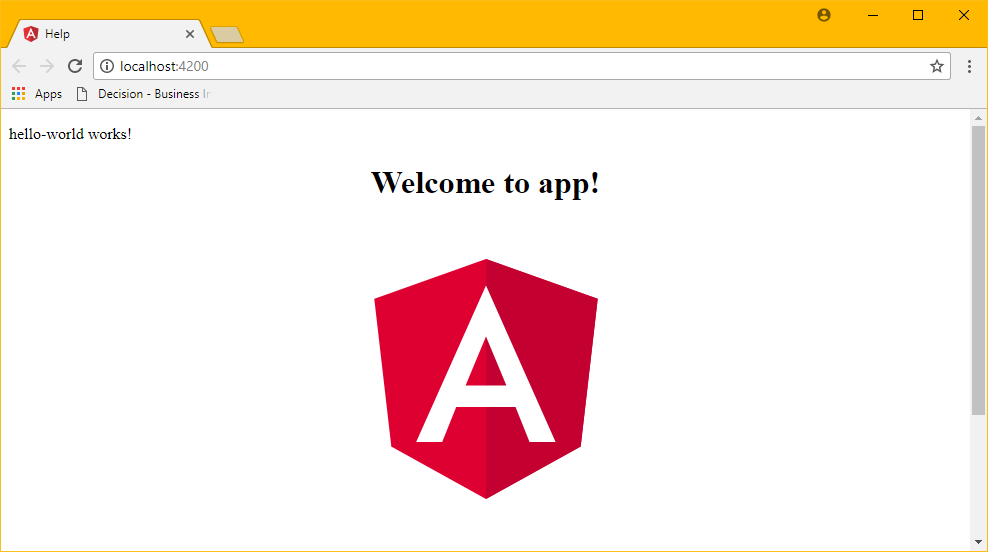
\includegraphics{images/hello-world-works.png}
\caption{}
\end{figure}

\chapter{Resources}\label{resources}

\section{Source Code}\label{source-code}

\subsection{angular-module-starter}\label{angular-module-starter}

The source code for the Angular Module Starter is available on
Github.com. You can use this Angular Custom Module project to start
building your own modules or as a reference. *
\url{https://github.com/buildmotion/angular-module-starter}

\section{Books}\label{books}

\subsection{Rangle's Angular 2 Training
Book}\label{rangles-angular-2-training-book}

\url{http://info.rangle.io/angular-2-training-book}

\section{Web}\label{web}

\subsection{Rangle.io Angular 2
Training}\label{rangle.io-angular-2-training}

\url{https://angular-2-training-book.rangle.io/}

\subsection{Angular.io Quickstart}\label{angular.io-quickstart}

\href{https://angular.io/guide/quickstart}{angular.io QuickStart}

\subsection{dofactory.com - Design
Patterns}\label{dofactory.com---design-patterns}

\url{http://www.dofactory.com}

\section{Design Patterns}\label{design-patterns}

\subsection{Facade Design Pattern}\label{facade-design-pattern}

\begin{itemize}
\tightlist
\item
  \url{https://en.wikipedia.org/wiki/Facade_pattern}
\item
  \url{http://www.dofactory.com/net/facade-design-pattern}
\end{itemize}

\section{Tools}\label{tools-1}

\subsection{Angular CLI}\label{angular-cli-1}

\url{https://cli.angular.io/}

\section{Testing}\label{testing}

\subsection{Specification Tests}\label{specification-tests}

\url{https://angular.io/guide/testing}

\bibliography{packages,book}


\end{document}
